\chapter{Background}
\label{background}

%intro to background
This project involved the use of protein interaction prediction to build weighted PPI networks improve the performance of a Community Detection algorithm on a PPI network.
%FIN: I'd probably explain the PPI acronym once more for people that skipped the beginning
The aim of the Community Detection algorithm was to gain insight into structure of the interactions between proteins at the synapse to aid disease research.
%FIN: you need to justify why the synapse is important in neuronal disease research with a reference at least
In the following chapter these different components, and how they fit together, will be described.

%what is a protein-protein interaction network?
\section{The synapse and protein interaction}

%intro paragraph, why proteins are important
Cells consist largely of proteins. 
%FIN: quantify - account for ~20% of the cell mass of a "typical eurkaryote" http://www.ncbi.nlm.nih.gov/books/NBK21473/
%FIN: "synthesis of proteins accounts for a considerable if highly variable proportion of the normal metabolism of a cell"  http://www.sciencedirect.com/science/article/pii/S1574789109000751
Each of these proteins are carefully tuned molecules which fit into machinery of a cell within the human body. %FIN: I dislike this sentence from an evolutionary perspective - plenty are shit - "Proteins facilitate almost every aspect of cellular metabolism across all forms of life.  They have evolved complex and extensive systems of interaction with one another and other cellular macro and micromolecules"
Functions of these cells include almost all cellular functions; there are proteins capable of pumping ions, reshaping DNA and fluorescing\autocite{alberts_molecular_2008}. %FIN:shoulda read the next sentence first before writing the last comment... still change that last 'tuned' sentence
A crude model of the cell is to map the interactions between these molecular machines to try to guess about the functioning of the cell. %FIN: explain why this is crude - it ignores the interaction of proteins with everything else!
These models are protein-protein interaction (PPI) networks and can be useful for disease research. %FIN: expand a little: how are they useful?  They allow targeted research, can identify additional previously uncharacterised disease factors, are targets for molecular therapies add a reference to one of the many PPI papers you are citing that explain why PPIs matter 

%going deeper, why do we care about proteins at the synapse, mention SYNSYS
The proteins at the synapse drive synaptic communication, which in turn defines the functioning of the brain.  %FIN: explain what the synapse is- the princpial interaction interface of a neuron - maybe move synapse section to before where yout alk about it
As these proteins define the functioning of the brain any disorders which affect the brain are very likely to involve these proteins.  %FIN: doesn't really justify why PPI itself is important though
Disorders which affect the brain are also very common and poorly understood, affecting one in three people in the developed world. %FIN: PPI offer opportunities to use known factors to identify additional uncharacterised protein factors in neuronal diseases
Curing these diseases therefore may be possible through a greater understanding of the interactions of proteins at the synaptic level\autocites{synsys,chua_architecture_2010}.

%what are synapses?
Synapses are the contacts between nerve cells where the vast majority of communication between nerve cells occurs, the only exceptions being through signalling molecules that can cross the cell membrane.
There are two types of synapses in the nervous system, electrical and chemical\autocite{kandel_principles_2000}.
Electrical synapses form a simple electrical connection through an ionic substrate between two neurons.
Chemical synapses are involved in a much more complex system of neurotransmitter release and reception.
Synapses are therefore important to the functioning of the nervous system. 
A problem with synapse function will likely cause large problems to the nervous system, so diseases of the nervous system are likely to involve problems with synapse function. %FIN: use the word neurotransmission its a great word, bonus points for 'impinge' 
As the cell is composed of proteins, so is the synapse composed of proteins. %FIN: there are lots of other shit too - I'd get rid of this its too simple in this form.  "As synapse function heavily features the interaction of many proteins e.g. transporters, signal-receptors, ... etc" - maybe choose some random specific examples
Investigating the functioning of these proteins will help to explain the functioning of the synapse and hopefully provide insight into the diseases of the synapse.%FIN:such as?  Some autistic spectrum disorders have been connected with heritable loss-of-function mutations in synaptic regulatory proteins such as Neuroglobin 4 http://jp.physoc.org/content/587/4/727

%but what is a protein-protein interaction network?
Physical interaction between proteins can be inferred from a range of different experiments.
Typical contemporary protein interaction networks rely on databases of confirmed interactions from a variety of experiments, for example in \textcite{kenley_detecting_2011} several well-known interaction databases were used. %FIN:give an example of one or two e.g. DIP and BioGRID 
By forming a network from these individual interactions as edges and clustering this network the example paper was able to predict complexes and functional associations. %FIN: example paper doesn't sound quite right - "Kenley et al. were able". Be more specific in what a functional association is
If these functional associations are involved in disease it is possible to associate proteins with diseases, as will be shown in section \ref{methods}. %FIN:how? If members of this functional association has been previously implicated in diseases or something

%historical work in the field
Originally, two papers, \textcite{ito_comprehensive_2001} and \textcite{uetz_comprehensive_2000}, were able to leverage large volumes of recent interaction data and build interaction networks. % mention they collected a lot of their own data in earlier papers by molecular methods (yeast-2h)
These papers were able to make interesting discoveries about the network of interactions in yeast simply by investigating subnetworks in the network that was produced.  %FIN: for example? identification of many previously unidentified proteins involved in yeast vesicular transport such as Ygl161c, Ygl198w, and Ylr324w

%which network are we interested in?
The interaction network we are investigating in this work is referred to throughout as the active zone network in the synapse.
These proteins are part of the pre-synapse and are illustrated in figure \ref{fig:actzone}.
Proteins identified as part of this network were used as baits in the pull-down experiments whose results are used in this project to build the PPI network which is the focus of the weighted and unweighted Community Detection.
%FIN: what is a pull-down experiment you still haven't explained it or why it is 'gold-standard' or that it is one of the gold-standards for demonstrating PPI in-vitro. Life scientists love to differentiate between in-vitro and in-vivo. While pull-down experiments can show interactions in-vitro (i.e. a test-tube) it doesn't necessarily mean the cells will interact in-vivo (in the cell).  That is why demonstrating that two proteins that interact also co-localise in the cell is important to confirm functional interaction.  Cells, and especially eukaryotic cells aren't really big bags of proteins (and other molecules) as they are often drawn in books - they contain a complex set of compartmentalisation, diffusion gradients and active retention or inactivation of proteins in certain areas

\begin{figure}
    \centering
    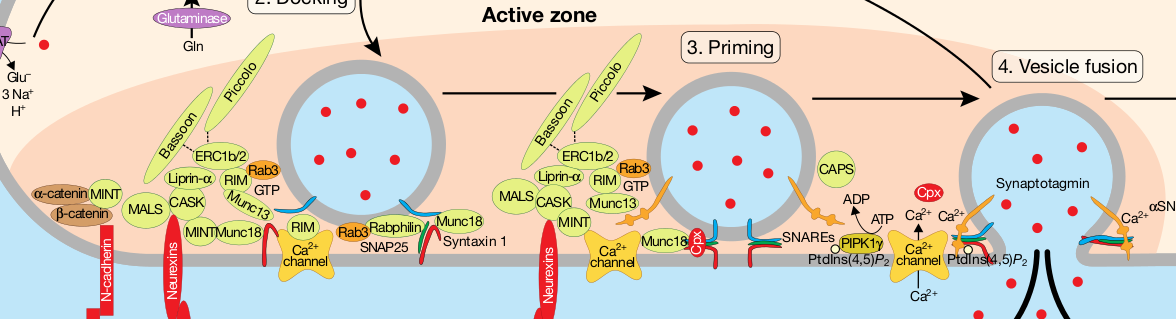
\includegraphics[width=\textwidth]{actzone.png}
    \caption{An illustration of the proteins identified to be involved in the active zone network\autocite{chua_architecture_2010}.}
    \label{fig:actzone}
\end{figure}

%function of the active zone network? What does it do?

%what is community detection?
\section{Protein complexes and community detection}

As mentioned in the previous section it is possible to analyse PPI networks to detect protein complexes and functional groups. %FIN: to identify predict PPI - unless you have proper co-localised interaction you can't say for certain they interact 
This has recently been achieved through use of Community Detection\autocites{chen_identifying_2013,wang_recent_2010}, which uses various methods to find community structure in graphs.

%what is community structure?
Community structure is described as a characteristic of graphs which have many connections within sub-groups but few connections outside that group\autocite{newman_communities_2012}.
Unfortunately, this description is not specific on exact measures for a graph to have community structure. %FIN: a little flippant - the specific criteria for a community in a graph is an open topic of discussion in the literature or something
Community detection algorithms are simply tested on graphs that are agreed to exhibit community structure with the aim of finding the pre-defined communities. %FIN: by whom, cite an example of one of these test graphs 

%describe how these algorithms usually work
There are two main approaches to the problem of Community Detection: traditional hierarchical methods and more recent optimization based methods\autocite{newman_communities_2012}.
Hierarchical methods were developed in the field of sociology and involves grading nodes by how highly connected they are in the network and then using this value to group nodes into communities.
Optimization based methods involves a different measure known as betweenness, which is analogous to the current flowing along edges if the graph were an electric circuit, and then allows a reductive technique where edges are removed iteratively to reveal sub-graphs without connections between them. %FIN:sentence needs fixed/split it too complex

%example paper using community detection on ppi graphs?
%FIN: http://www.biomedcentral.com/1752-0509/4/100/ 

%what is protein-protein interaction prediction?
\section{Protein-protein interaction prediction}

Protein interaction prediction was developed to solve the problem of incomplete and unreliable interaction data by combining both direct and indirect information\autocite{qi_learning_2008}.
Direct information are the result of experiments, such as yeast two-hybrid, intended to directly find protein-protein interactions.  %FIN: explain what y2h is and why it is good - you reconstitute some split marker (transcription factor or something) only when two proteins interact from 2 genetically modified yeast hybrids. So if you see that marker it means that the proteins you've put in each hybrid interact
Indirect information includes biological data that was not gathered directly to find interactions, such as gene expression data. %FIN: explain; two proteins can only interact if they are both expressed at the same time and place within a cell therefore co-expression and co-localisation data are important sources of indirect evidence for PPI (in fact are necessary for true PPI)
More information on the data sources can be found in the following section \ref{back:sources}.


%what are features?
To predict a protein interaction we need to have a value or sequence of values from which to make our guess as to the existence of an interaction.
For each interaction this set of values are known as features.
The bulk of the work in this project involved obtaining these values for every feature necessary to train the classifier and classify the interactions of the synaptic network.  %FIN: maybe expand on this being non-trivial due to the plethora of data sources and alternative identifiers they use. 

%what is the classifier
The classifier is a machine learning algorithm that can learn from a labelled training set how to sort these vectors of features into the appropriate category. %citation to Murphy?  %FIN: citation to the Murphy's law might be appropriate... 
However, these algorithms cannot make predictions unless the training data is informative.   
Also, the training data must be an accurate representation of the case the algorithm is planned to be applied to. %FIN:make this specific to your data as well - so for example the training data must use validated examples of protein protein interactions 

%why do we want to predict protein-protein interactions?
%reference to ENTS and similar projects aiming to make full interactomes
%how this is different to our goal
Completing the interactome of a given organism from incomplete data is a major goal for some works in the protein interaction field, such as \textcite{rodgers-melnick_predicting_2013}.
The goal in this project is to appropriately weight interactions in a PPI network to improve the performance of a Community Detection algorithm.

%what's the point in weighting connections?
Weakly interacting proteins will have a lower confidence in their interacting at all, as it will have been observed less frequently.
Therefore, by weighting the interactions in a PPI network according to our confidence we can also make the PPI network reflect more closely the true situation. %FIN: i.e. proteins predicted to interact actually interacting in vivo 

%what data sources were used to predict protein-protein interactions?
\section{Data sources and networks}
\label{back:sources}

%Different types of sources used with reference to other works
Many different data sources were considered for inclusion in this project. %FIN: such as - which ones haven't been mentioned in the table - that you considered but discarded 
The full list can be found in Appendix \ref{datasources}.
These different data sources fall into categories described in table \ref{tab:sources}.

\begin{table}
    \centering
    \small
    \begin{tabular}{p{0.2\textwidth} p{0.5\textwidth}}
        Data source type                                & Examples \\
        \hline
        \multirow{3}{*}{\parbox{0.2\textwidth}{Primary interaction databases}}  & DIP\autocite{xenarios_dip_2002} \\
                                                        & HIPPIE\autocite{schaefer_hippie:_2012} \\ 
                                                        & BioGRID\autocite{stark_biogrid:_2006} \\
        \hline
        \multirow{2}{*}{\parbox{0.2\textwidth}{Associated features}}            & Features derived from Gene Ontology\autocite{ashburner_gene_2000} \\
                                                        & Those used in \textcite{rodgers-melnick_predicting_2013} \\
        \hline
        \multirow{2}{*}{\parbox{0.2\textwidth}{Other PPI prediction resources}} & STRING\autocite{von_mering_string:_2005} \\
                                                        & InterologWalk\autocite{gallone_bio::homology::interologwalk_2011} \\
    \end{tabular}
    \caption{A table summarising the different sources of data used in the course of the project.}
    \label{tab:sources}
\end{table}

%why they were chosen
The indirect sources of data were chosen based on usage in the literature, such as in the case of Gene Ontology\autocite{qi_evaluation_2006}. 
Direct data sources were listed by investigating all of the available databases which could be of use and choosing from these.
%FIN: this is weak and needs expanded on - evaluation of different data sources and issues you had getting them were a major part of the work in this project - some data sources were poorly accessible or standardised - give examples. Some weren't informative etc.  Justify why GO terms could be useful (co-localisation and co-functionalisation information more likely to interact)
\section*{Conclusion}

The goal of this project involved obtaining weights for a PPI network correlated with the strength of different protein interactions to improve the performance of a Community Detection algorithm.
Improving the performance in this way, it was hoped would produce new insight into protein interactions that could cause disease.


